\section{Reverse square function estimate for the cone in $\R^{2+1}$}

For a dyadic number $\delta\in 2^{-\Z}$ we denote by $\Part{\delta}$ a boundedly overlapping covering of the truncated cone $\calC$ in $\R^{2+1}$ by adapted $1 \times \delta^{1/2} \times \delta$-slabs (TODO: change to $1 \times \delta \times \delta^{2}$).
One can think of them as being associated to arcs of angular length $2\pi \delta$ on the circle, but such dyadic structure is not preserved by affine scaling that we will use.
We fix partitions
\[
\Part{\delta/2} = \cup_{\theta \in \Part{\delta}} \Part[\theta]{\delta/2}
\]
such that $\theta' \in \Part[\theta]{\delta/2}$ only if $\theta'\cap\theta\neq\emptyset$.
Then for any $\delta' < \delta$ and $\theta \in \Part{\delta}$ we can define $\Part[\theta]{\delta'}$ in such a way that for $\delta''<\delta'<\delta$ we have
\[
\Part[\theta]{\delta''} = \cup_{\theta' \in \Part[\theta]{\delta'}} \Part[\theta']{\delta''}.
\]
Given $f_{\theta}$ for $\theta \in \Part{\delta_{0}}$ with $\supp \widehat{f_{\theta}} \subseteq \theta$ for some small $\delta_{0}$ we define for $\delta_{0} < \delta \leq 1$ and $\tau\in\Part{\delta}$
\[
f_{\tau} := \sum_{\theta \in \Part[\tau]{\delta_{0}}} f_{\theta},
\quad
f := \sum_{\theta \in \Part{\delta_{0}}} f_{\theta}.
\]
Let us denote by $\RvSq^{p}(\delta)$ (for ``reverse square function estimate'') the smallest constant such that the estimate
\begin{equation}
\label{eq:RvSq:def}
\norm{f}_{p} \leq
\RvSq^{p}(\delta) \norm{ \ell^{2}_{\theta \in \Part{\delta}} f_{\theta} }_{p}
\end{equation}
holds for any $f_{\theta}$ as above.

\subsection{Lorentz scaling}
The cone has a scaling symmetry similar to that of the parabola.
Let $0<\gamma<1/100$ be a small number and $T : \R^3 \to \R^3$ be the linear transformation given by
\[
T(1,0,1) = (1,0,1),
\quad T(-1,0,1) = \gamma^{2}(-1,0,1),
\quad T(0,1,0) = \gamma(0,1,0).
\]
Then in the standard coordinates $T$ is given by the matrix
\[
\begin{pmatrix}
\frac{1+\gamma^{2}}{2} & 0 & \frac{1-\gamma^{2}}{2}\\
0 & \gamma & 0\\
\frac{1-\gamma^{2}}{2} & 0 & \frac{1+\gamma^{2}}{2}
\end{pmatrix},
\]
and one can verify that it preserves the cone given by the equation $\xi_{1}^{2}+\xi_{2}^{2}=\xi_{3}^{2}$.
Also, it maps the $\delta/\gamma^{2}$-neighborhood of the truncated cone sector
\[
\Set{ (\xi,\abs{\xi} ) \given \xi\in\R^{2}, 1/2 \leq \abs{\xi} \leq 4, \xi_{1}>1/2 }
\]
onto the $\delta$-neighborhood of a sector of the truncated cone $\calC$ of width $\sim\gamma$ near $(1,0,1)$.

Let $\tau \in \Part{\gamma^{2}}$ be the slab pointing in the direction $(1,0,1)$ and $\theta\in\Part[\tau]{\delta}$.
Then $T^{-1}\theta$ is a slab of scale $\delta/\gamma^{2}$ adapted to the cone.
We apply \eqref{eq:RvSq:def} to the functions $f_{\theta} \circ T^{-t}$.
Since $\widehat{f_{\theta} \circ T^{-t}} = \abs{\det T} \widehat{f_{\theta}} \circ T$ we obtain
\begin{equation}
\label{eq:RvSq:scaling}
\norm{f_{\tau}}_{p}
\lesssim
\RvSq^{p}(\delta/\gamma^{2}) \norm{\ell^{2}_{\theta \in \Part[\tau]{\delta}} f_{\theta}}_{p}.
\end{equation}
By rotation invariance this estimate continues to hold for arbitrary $\tau \in \Part{\gamma^{2}}$.
Abusing notation we will write
\[
S_{\delta}f := \ell^{2}_{\theta\in\Part{\delta}} f_{\theta},
\quad
S_{\delta}f_{\tau} := \ell^{2}_{\theta\in\Part[\tau]{\delta}} f_{\theta}.
\]

\subsection{Multilinear reverse square function estimate}

\subsubsection{Transversality}
Let $\calC_{\tau} := \calC \cap 5 \tau$ be the piece of the truncated cone close to $\tau \in \Part{\gamma}$.
Denote by $N(\xi)$ the unit normal vector to $\calC$ at $\xi$ (say, inward).
We call $\tau_{1},\tau_{2},\tau_{3} \in \Part{\gamma}$ \emph{$\nu$-transverse} if for every $\xi_{i} \in \calC_{\tau_{i}}$ we have
\begin{equation}
\label{eq:cone-transversality}
\abs{ N(\xi_{1}) \wedge N(\xi_{2}) \wedge N(\xi_{3}) } \geq \nu,
\end{equation}
see Figure~\ref{fig:transverse}.
A key geometric property of the cone $\calC$ is that if $\tau_1, \tau_2, \tau_3 \in \Part{\gamma}$ are mutually separated by a distance $d > 10 \gamma^{1/2}$, then they are $cd^{3}$-transverse.
To see this notice that for $\xi\in\R^{2}$ we have $N((\xi,{\abs{\xi}}))=(-\xi/\abs{\xi},1)$, so we wedge product in \eqref{eq:cone-transversality} is proportional to the area of a certain triangle by the same computation as for the paraboloid in $\R^{3+1}$.
This triangle has side lengths $\gtrsim d$ and vertices on the unit circle, so its area is $\gtrsim d^{3}$.

%
\begin{figure}
\begin{center}
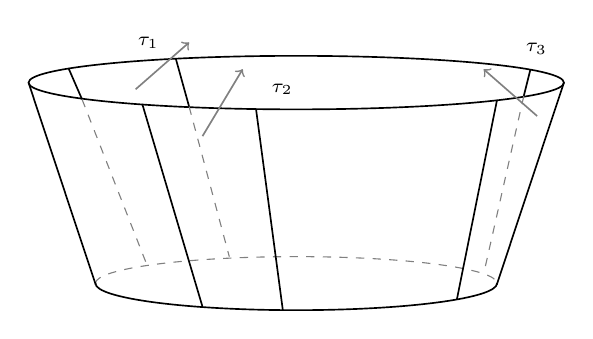
\begin{tikzpicture}[scale = 1.7]
	\draw[semithick] (4,1.5) ellipse (2 and 0.2);
	\draw[semithick] (2.5,0) arc (180:360:1.5 and 0.2);
	\draw[dashed,color=gray] (2.5,0) arc (180:0:1.5 and 0.2);
	\draw[semithick] (2.502,-0.01) -- (2,1.5);
	\draw[semithick] (5.498,-0.01) -- (6,1.5);
	%
	\draw[semithick] (3.3,-0.175) -- (2.85,1.34);
	\draw[semithick] (3.9,-0.2) -- (3.7,1.3);
	\draw[->,semithick,color=gray] (3.3,1.1) -- (3.6,1.6);
	\draw (3.9,1.45) node {$\calC_{\tau_2}$};
	%
	\draw[semithick] (3.1,1.68) -- (3.2,1.32);
	\draw[dashed,color=gray] (3.2,1.32) -- (3.5,0.2);
	\draw[semithick] (2.3,1.605) -- (2.4,1.375);
	\draw[dashed,color=gray] (2.4,1.375) -- (2.88,0.15);
	\draw[->,semithick,color=gray] (2.8,1.45) -- (3.2,1.8);
	\draw (2.9,1.8) node {$\calC_{\tau_{1}}$};
	%
	\draw[semithick] (5.2,-0.12) -- (5.5,1.37);
	\draw[semithick] (5.7,1.4)-- (5.75,1.6);
	\draw[dashed,color=gray] (5.7,1.4) -- (5.4,0.07);
	\draw[->,semithick,color=gray] (5.8,1.25) -- (5.4,1.6);
	\draw (5.8,1.75) node {$\calC_{\tau_3}$};
\end{tikzpicture}
\end{center}
\caption{Transverse sectors on the cone (copied from \cite{arxiv:1607.08426}).}
\label{fig:transverse}
\end{figure}

We will denote by $\MlRvSq^{p}(\delta,\gamma)$ (for ``multilinear reverse square function estimate'') the smallest constant such that the estimate
\begin{equation}
\label{eq:MlRvSq:def}
\norm[\Big]{ \avprod_{i=1}^{3} \abs{f_{\tau_{i}}} }_p
\leq \MlRvSq^{p}(\delta,\gamma)
\avprod_{i=1}^{3} \norm{S_\delta f_{\tau_{i}} }_p
\end{equation}
holds for all $10\gamma^{1/2}$-separated triples $\tau_{1},\tau_{2},\tau_{3} \in \Part{\gamma}$.
By H\"older's inequality we have $\MlRvSq^{p}(\delta,\gamma) \leq \RvSq^{p}(\delta)$.
We will now show a converse estimate.

\subsubsection{Bourgain--Guth argument}
The statement below is a simplified version of \cite[(23)]{MR2927399}.
\begin{lem}
\label{lem:LinTriLcompare}
Let $0 < \gamma < 1$.
Then for any $x \in \R^3$,
\begin{equation}
\label{eq:BG-arg-cone2+1}
\abs{ f(x) } \lesssim
\max \Bigl(
\max_{\tau \in \Part{\gamma}}\abs{ f_{\tau}(x) },
\gamma^{-1}
\max_{\substack{\tau_1,\tau_2,\tau_3 \in \Part{\gamma}: \\ \dist(\tau_i, \tau_j) \ge 10\gamma,\, i\neq j}}
\prod_{i=1}^{3} \abs{f_{\tau_i}(x)}^{1/3} \Bigr).
\end{equation}
\end{lem}
\begin{proof}
If
\[
\abs{ f(x) } \leq C \max_{\tau \in \Part{\gamma}}\abs{ f_{\tau}(x) },
\]
then we are done.
Otherwise we have
\[
\sum_{\tau \in \Part{\gamma}}\abs{ f_{\tau}(x) }
\geq
\abs{ f(x) }
\geq
C \max_{\tau \in \Part{\gamma}}\abs{ f_{\tau}(x) },
\]
and since $\#\Part{\gamma} \sim \gamma^{-1/2}$ it follows that
\[
\# \Set{ \tau \in \Part{\gamma} \given \abs{ f_{\tau}(x) } \geq c\gamma^{1/2} \max_{\tau \in \Part{\gamma}}\abs{ f_{\tau}(x) } }
\geq
C
\]
for a small absolute constant $c>0$ and a large absolute constant $C$.
If the latter constant is large enough, then we can choose $10 \gamma$-separated $\tau_{1},\tau_{2},\tau_{3}$ from this set, and with this choice we have
\[
\abs{ f(x) }
\leq
\sum_{\tau \in \Part{\gamma}}\abs{ f_{\tau}(x) }
\lesssim
\gamma^{-1/2} \max_{\tau \in \Part{\gamma}}\abs{ f_{\tau}(x) }
\lesssim
\gamma^{-1} \prod_{i=1}^{3} \abs{f_{\tau_i}(x)}^{1/3}.
\qedhere
\]
\end{proof}
\begin{remark}
A slightly more careful argument shows that $\gamma^{-1}$ can be replaced by $\gamma^{-1/2}$ in \eqref{eq:BG-arg-cone2+1}.
\end{remark}
Using Lemma~\ref{lem:LinTriLcompare} we can establish the following relation between the linear and trilinear square function estimates.

\begin{prop} \label{prop:MSQmeanSQ}
Let $p \ge 2$.
The for every $0<\gamma<1$ we have
\begin{equation}
\label{eq:RvSq-vs-MlRvSq}
\RvSq^{p}(\delta)
\lesssim
\RvSq^{p}(\delta / \gamma^2) + \gamma^{-2-3/(2p)} \MlRvSq^{p}(\delta,\gamma)
\end{equation}
with the implicit constant independent of $\gamma$.
\end{prop}

\begin{proof}
Fix $\gamma$ and $f_{\theta}$.
Raising the estimate~\eqref{eq:BG-arg-cone2+1} to the power $p$, replacing maximum by a sum, and integrating over $\R^{2+1}$ we obtain
\begin{equation} \label{LpTricom}
\begin{split}
\norm{ f }_p^p
&\lesssim \sum_{\tau \in \Part{\gamma}} \norm{ f_{\tau} }_p^p
+ \gamma^{-2p}
\sum_{\substack{\tau_1,\tau_2,\tau_3 \in \Part{\gamma}: \\ \dist(\tau_i, \tau_j) \ge 10\gamma,\, i\neq j}}
\norm[\Big]{ \prod_{i=1}^{3} \abs{f_{\tau_i}}^{1/3} }_p^p.
\end{split}
\end{equation}

Consider the first sum on the right-hand side of \eqref{LpTricom}.
By \eqref{eq:RvSq:scaling} we have
\begin{equation} \label{ppsc}
\norm{ f_\tau }_p
\lesssim \RvSq^{p}(\delta / \gamma^2)
\norm{ \ell^{2}_{\theta\in\Part[\tau]{\delta}} f_{\tau} }_p.
\end{equation}
For $p \ge 2$ we have
\begin{align*}
\ell^{p}_{\tau \in \Part{\gamma}} \norm{ \ell^{2}_{\theta\in\Part[\tau]{\delta}} f_{\theta} }_p
&=
\norm{ \ell^{p}_{\tau \in \Part{\gamma}} \ell^{2}_{\theta\in\Part[\tau]{\delta}} f_{\theta} }_p\\
&\leq
\norm{ \ell^{2}_{\tau \in \Part{\gamma}} \ell^{2}_{\theta\in\Part[\tau]{\delta}} f_{\theta} }_p\\
&=
\norm{ \ell^{2}_{\theta\in\Part{\delta}} f_{\theta} }_p.
\end{align*}

Consider the trilinear term on the right-hand side of \eqref{LpTricom}.
By definition \eqref{eq:MlRvSq:def} we have
\begin{align*}
\sum_{\substack{\tau_1,\tau_2,\tau_3 \in \Part{\gamma}: \\ \dist(\tau_i, \tau_j) \ge 10\gamma,\, i\neq j}}
\norm[\Big]{ \avprod_{i=1}^{3} \abs{f_{\tau_i}} }_p^p
&\leq
\sum_{\substack{\tau_1,\tau_2,\tau_3 \in \Part{\gamma}: \\ \dist(\tau_i, \tau_j) \ge 10\gamma,\, i\neq j}}
\MlRvSq^{p}(\delta,\gamma)^{p} \avprod \norm{\ell^{2}_{\theta\in\Part[\tau_{i}]{\delta}} f_{\theta}}^{p}\\
&\leq
\sum_{\tau_1,\tau_2,\tau_3 \in \Part{\gamma}}
\MlRvSq^{p}(\delta,\gamma)^{p} \avprod \norm{\ell^{2}_{\theta\in\Part{\delta}} f_{\theta}}^{p}\\
&\lesssim
\gamma^{-3/2} \MlRvSq^{p}(\delta,\gamma)^{p} \norm{\ell^{2}_{\theta\in\Part{\delta}} f_{\theta}}^{p}.
\end{align*}

Substituting these estimates in \eqref{LpTricom} we obtain
\[
\norm{f}_p
\lesssim
\bigl( \RvSq^{p}(\delta / \gamma^2) + \gamma^{-2-3/(2p)} \MlRvSq^{p}(\delta,\gamma) \bigr)
\norm{\ell^{2}_{\theta\in\Part{\delta}} f_{\theta}}.
\]
Since $f_{\theta}$ were arbitrary this gives the claim.
\end{proof}

\begin{corollary}
\label{cor:RvSq-vs-MlRvSq}
Let $2 \leq p < \infty$ and $\alpha > 0$.
If $\MlRvSq^{p}(\delta,\gamma) \lesssim_{\gamma} \delta^{-\alpha}$ holds for all $0< \gamma < 1$, then $\RvSq^{p}(\delta) \lesssim_{\epsilon} \delta^{-\alpha-\epsilon}$ holds for all $\epsilon>0$.
\end{corollary}
The proof is the same as for decoupling: choose $\gamma$ small and iterate \eqref{eq:RvSq-vs-MlRvSq}.

\subsection{The $L^{3}(\R^{2+1},\ell^{2})$ estimate}
In this section we prove the following result.
\begin{theorem}[{\cite{MR2927399}}]
\label{thm:RvSq:L3}
For every $\epsilon>0$ we have
\begin{equation}
\label{eq:RvSq:L3}
\RvSq^{3}(\delta) \lesssim_{\epsilon} \delta^{-\epsilon}.
\end{equation}
\end{theorem}
Theorem~\ref{thm:RvSq:L3} implies the sharp local smoothing estimate for the wave equation on $L^{3}(\R^{2})$.

\subsubsection{Multilinear restriction}
Let $\tau_{1},\tau_{2},\tau_{3} \in \Part{\gamma}$ be $10\gamma$-separated.
By multilinear restriction on a ball $B \subset \R^{3}$ of radius $\delta^{-1/2}$ we have
\begin{equation}
\label{eq:MlRvSq:multRestr:ball}
\norm[\big]{ \avprod f_{\tau_{i}} }_{L^{3}(B)}
\lesssim_{\gamma,\epsilon}
\delta^{1/4-\epsilon} \avprod \norm{f_{\tau_{i}} \psi_{B}}_{2},
\end{equation}
were $\psi_{B}$ is a bump function adapted to $B$ with Fourier support in $B(0,\delta^{1/2})$, since
\[
\supp \widehat{ f_{\tau_{i}} \psi_{B} }
\subseteq
\supp \widehat{ f_{\tau_{i}} } + \supp \widehat{ \psi_{B} }
\]
is contained in the $\delta^{1/2}$-neighborhood of the cone.

Taking the $\ell^{3}_{B}$ norm over a finitely overlapping covering of $\R^{3}$ by balls of radius $\delta^{-1/2}$ and applying H\"older's inequality we obtain
\begin{equation}
\label{eq:MlRvSq:multRestr}
\norm[\big]{ \avprod f_{\tau_i} }_{3}
\sim
\ell^{3}_{B} \norm[\big]{ \avprod f_{\tau_i} }_{L^3(B)}
\lesssim_{\gamma,\epsilon} \delta^{1/4-\epsilon/2} \avprod \ell^{3}_{B} \norm{f_{\tau_i} \psi_{B}}_{2}.
\end{equation}

\subsubsection{Orthogonality}
Since the $\delta^{1/2}$-neighborhoods of $\theta \in \Part{\delta}$ have bounded overlap, by almost orthogonality we have
\[
\norm{f_{\tau_i} \psi_{B}}_{2}
\lesssim
\norm{ \ell^{2}_{\theta \in \Part[\tau_{i}]{\delta}} ( f_{\theta} \psi_B ) }_{2}
\lesssim
\norm{ \ell^{2}_{\theta \in \Part[\tau_{i}]{\delta}} f_{\theta} }_{L^2(w_B)}.
\]
By this estimate and H\"older's inequality,
\begin{multline}
\ell^{3}_{B}\norm{f_{\tau_i} \psi_{B}}_{2}
\lesssim
\ell^{3}_{B}\norm{S_\delta f_{\tau_i}}_{L^2(w_{B})}\\
\lesssim
\delta^{-\frac{3}{2}\big( \frac{1}{2} - \frac{1}{3} \big)} \ell^{3}_{B} \norm{S_\delta f_{\tau_i}}_{L^3(w_{B})}
\lesssim
\delta^{-\frac{1}{4}} \norm{ S_\delta f_{\tau_i}}_{L^{3}(\R^{3})}.
\end{multline}
Substituting this in \eqref{eq:MlRvSq:multRestr} and taking the supremum over $f_{\theta}$ we obtain
\[
\MlRvSq^{3}(\delta,\gamma)
\lesssim_{\gamma,\epsilon} \delta^{-\epsilon}.
\]
Theorem~\ref{thm:RvSq:L3} follows by Corollary~\ref{cor:RvSq-vs-MlRvSq}.

\subsection{The $L^{p}(\R^{2+1}, \ell^{2})$ estimate}
\begin{theorem}[{cf.\ \cite{arxiv:1607.08426}}]
Let $3 \leq p \leq 6$ and $\alpha = \frac{(p-2) ( p - 3 )}{2 p^{2}}$.
Then for every $\epsilon>0$ we have
\begin{equation}
\label{eq:RvSq:Lp}
\RvSq^{p}(\delta)
\lesssim_{\epsilon}
\delta^{-\alpha-\epsilon}.
\end{equation}
\end{theorem}
In \cite{arxiv:1607.08426} this is proved for $p=4$ and we follow the argument given there.
It is somewhat surprising that the resulting exponent $\alpha$ is not an affine function of $1/p$.
In particular, for intermediate exponents this is better than what interpolation between cases $p=3,4,6$ would give.
For $3<p<4$ this gives a small improvement over \cite[Figure 7]{arxiv:1812.11616}.
The local smoothing conjecture for the wave equation in $\R^{2+1}$ would follow from \eqref{eq:RvSq:Lp} with $p=4$ and $\alpha=0$.

\subsubsection{Multilinear restriction}
Let again $\tau_{1},\tau_{2},\tau_{3} \in \Part{\gamma}$ be $10\gamma$-separated and consider a ball $B \subset \R^{3}$ of radius $\delta^{-\kappa}$.
%\eqref{eq:MlRvSq:multRestr:ball}
By multilinear restriction we have
\[
\norm[\big]{ \avprod f_{\tau_i} }_{L^{3}(B)}
\lesssim_{\epsilon}
\delta^{\kappa/2 -\epsilon} \avprod \norm{f_{\tau_i}}_{L^{2}(\R^{3})}
\]
for all $f_{\tau_i}$ with Fourier support in $\delta^{\kappa}$-neighborhoods of $\calC_{\tau_{i}}$.
By orthogonality
\[
\norm{ f }_2
\lesssim
\ell^{2}_{\tau \in \Part[\tau_{i}]{\delta^{\kappa}}} \norm{ f_{\tau} }_2.
\]
Thus, we have
\begin{equation*}
\norm[\big]{ \avprod f_{\tau_i} }_{L^{3}(B)}
\lesssim_\epsilon
\delta^{\kappa/2-\epsilon} \avprod \ell^{2}_{\tau \in \Part[\tau_{i}]{\delta^{\kappa}}} \norm{f_{\tau}}_{2}.
\end{equation*}
By H\"older's inequality and decoupling we have
\[
\norm[\big]{ \avprod f_{\tau_i} }_{L^{6}(B)}
\leq
\avprod \norm{ f_{\tau_i} }_{L^{6}(B)}
\lesssim_\epsilon
\delta^{-\epsilon} \avprod \ell^{2}_{\tau \in \Part[\tau_{i}]{\delta^{\kappa}}} \norm{f_{\tau}}_{6}.
\]
The last two displays hold for arbitrary functions with $\supp \widehat{f_{\tau}} \subseteq \tau$ for $\tau \in \Part{\delta^{\kappa}}$, not necessarily of the form $f_{\tau} = \sum_{\theta\in\Part[\tau]{\delta}} f_{\theta}$.
Define $\theta,q,\beta$ by
\[
\frac{1}{p} = \frac{\theta}{3} + \frac{1-\theta}{6},
\quad
\frac{1}{q} = \frac{\theta}{2} + \frac{1-\theta}{6},
\quad
\frac{1}{q} = \frac{\beta}{2} + \frac{1-\beta}{p}.
\]
Then by complex interpolation
\[
\norm[\big]{ \avprod f_{\tau_i} }_{L^{p}(B)}
\lesssim_\epsilon
\delta^{\theta \kappa/2-\epsilon} \avprod \ell^{2}_{\tau \in \Part[\tau_{i}]{\delta^{\kappa}}} \norm{f_{\tau}}_{q}.
\]
Replacing each $f_{\tau}$ by $f_{\tau}\psi_{B}$, where $\psi_{B}$ is an $L^{\infty}$ normalized bump function adapted to $B$ with Fourier support in $B(0,\delta^{\kappa})$ we obtain
\begin{align*}
\norm[\big]{ \avprod f_{\tau_i} }_{L^{p}(B)}
&\lesssim
\norm[\big]{ \avprod (f_{\tau_i}\psi_{B}) }_{L^{p}(B)}\\
&\lesssim_{\epsilon}
\delta^{\theta \kappa/2-\epsilon} \avprod \ell^{2}_{\tau \in \Part[\tau_{i}]{\delta^{\kappa}}} \norm{f_{\tau}\psi_{B}}_{q}
\end{align*}
By H\"older's inequality this implies
\begin{equation}
\norm[\big]{ \avprod f_{\tau_i} }_{L^{p}(B)}
\lesssim_\epsilon
\delta^{\theta \kappa/2-\epsilon} \avprod \Big( \ell^{2}_{\tau \in \Part[\tau_i]{\delta^{\kappa}}} \norm{f_{\tau} \psi_{B}}_{p} \Big)^{1-\beta}
\Big( \ell^{2}_{\tau \in \Part[\tau_i]{\delta^{\kappa}}} \norm{f_{\tau} \psi_{B}}_{2} \Big)^{\beta}.
\end{equation}
By H\"older's inequality we obtain
\begin{multline}
\label{eq:jlee-dec}
\norm[\big]{ \avprod f_{\tau_i} }_{L^{p}(\R^{3})}
\sim
\ell^{p}_{B} \norm[\big]{ \avprod f_{\tau_i} }_{L^{p}(B)}
\lesssim_\epsilon
\delta^{\theta \kappa/2-\epsilon} \avprod \Big( \ell^{p}_{B} \ell^{2}_{\tau \in \Part[\tau_i]{\delta^{\kappa}}} \norm{f_{\tau} \psi_{B}}_{p} \Big)^{1-\beta}\\
\cdot \Big( \ell^{p}_{B} \ell^{2}_{\tau \in \Part[\tau_i]{\delta^{\kappa}}} \norm{f_{\tau} \psi_{B}}_{2} \Big)^{\beta}.
\end{multline}
Now we specify to $\kappa=1/2$ and functions of the form $f_{\tau} = \sum_{\theta\in\Part[\tau]{\delta}} f_{\theta}$.

\subsubsection{Orthogonality}
For each $\theta\in\Part{\delta}$ the Fourier support of $f_{\theta} \psi_B$ is contained in the $\delta^{1/2}$-neighborhood of $\theta$, and these neighborhoods have bounded overlap (here we need $\kappa\geq 1/2$).
Hence
\begin{multline*}
\ell^{2}_{\tau \in \Part[\tau_i]{\delta^{1/2}}} \norm{f_{\tau} \psi_{B}}_{2}
=
\ell^{2}_{\tau \in \Part[\tau_i]{\delta^{1/2}}} \norm{\sum_{\theta \in \Part[\tau]{\delta}}f_{\theta} \psi_{B}}_{2}\\
\lesssim
\ell^{2}_{\tau \in \Part[\tau_i]{\delta^{1/2}}} \ell^{2}_{\theta \in \Part[\tau]{\delta}} \norm{ f_{\theta} \psi_{B}}_{2}
=
\ell^{2}_{\theta \in \Part[\tau_i]{\delta}} \norm{ f_{\theta} \psi_{B}}_{2}
\lesssim
\norm{ S_{\delta} f_{\tau_{i}} }_{L^{2}(w_{B})}.
\end{multline*}
By this estimate and H\"older's inequality
\begin{multline}\label{L2part}
\ell^{p}_{B} \ell^{2}_{\tau \in \Part[\tau_i]{\delta^{1/2}}} \norm{f_{\tau} \psi_{B}}_{2}
\lesssim
\ell^{p}_{B} \norm{S_\delta f_{\tau_i}}_{L^2(w_{B})}\\
\lesssim
\delta^{-\frac{3}{2}\big( \frac{1}{2} - \frac{1}{p} \big)} \ell^{p}_{B} \norm{S_\delta f_{\tau_i}}_{L^p(w_{B})}
\lesssim
\delta^{-\frac{3}{2}\big( \frac{1}{2} - \frac{1}{p} \big)} \norm{ S_\delta f_{\tau_i}}_{p}.
\end{multline}


\subsubsection{Scaling}
Let $\alpha \ge 0$ be the smallest number such that \eqref{eq:RvSq:Lp} holds for all $\epsilon>0$.
By Minkowski's inequality
\[
\ell^{p}_{B} \ell^{2}_{\tau \in \Part[\tau_i]{\delta^{1/2}}} \norm{f_{\tau} \psi_{B}}_{p}
\lesssim
\ell^{2}_{\tau \in \Part[\tau_i]{\delta^{1/2}}} \ell^{p}_{B} \norm{f_{\tau}}_{L^{p}(w_{B})}
\sim
\ell^{2}_{\tau \in \Part[\tau_i]{\delta^{1/2}}} \norm{f_{\tau}}_{p}.
\]
By Lorentz scaling \eqref{eq:RvSq:scaling} we have
\[
\norm{ f_{\tau} }_p
\lesssim_\epsilon
\delta^{-\alpha/2 - \epsilon} \norm{ S_\delta f_{\tau} }_p.
\]
Inserting this and \eqref{L2part} into \eqref{eq:jlee-dec} we obtain
\[
\norm[\big]{ \avprod f_{\tau_i} }_{L^{p}(\R^{3})}
\lesssim_\epsilon
\delta^{\theta/4-\epsilon} \avprod \Big( \delta^{-\alpha/2} \ell^{2}_{\tau \in \Part[\tau_i]{\delta^{1/2}}} \norm{ S_\delta f_{\tau} }_p \Big)^{1-\beta}\\
\cdot \Big( \delta^{-\frac{3}{2} \bigl( \frac{1}{2} - \frac{1}{p} \bigr)} \norm{ S_\delta f_{\tau_i} }_p \Big)^{\beta}.
\]
Since
\[
\beta(1/2-1/p)=(1/q-1/p)=\theta/2-\theta/3=\theta/6
\]
it follows that
\[
\norm[\big]{ \avprod f_{\tau_i} }_{L^{p}(\R^{3})}
\lesssim_\epsilon
\delta^{-\alpha(1-\beta)/2-\epsilon} \avprod \Big( \ell^{2}_{\tau \in \Part[\tau_i]{\delta^{1/2}}} \norm{ S_\delta f_{\tau} }_p \Big)^{1-\beta}\\
\cdot \norm{ S_\delta f_{\tau_i} }_p^{\beta}.
\]
By doing the bootstrapping argument more carefully we should be able to obtain a hybrid between decoupling and square function inequalities starting from here.
However, we want everything to be in terms of square functions, so we estimate
\begin{align*}
\ell^{2}_{\tau \in \Part[\tau_i]{\delta^{1/2}}} \norm{ S_\delta f_{\tau} }_p
&\lesssim
\delta^{-\frac{1}{4} \big( \frac{1}{2} - \frac{1}{p} \big)}
\ell^{p}_{\tau \in \Part[\tau_i]{\delta^{1/2}}} \norm{ S_\delta f_{\tau} }_p\\
&=
\delta^{-\frac{1}{4} \big( \frac{1}{2} - \frac{1}{p} \big)}
\norm{ \ell^{p}_{\tau \in \Part[\tau_i]{\delta^{1/2}}} S_\delta f_{\tau} }_p\\
&\leq
\delta^{-\frac{1}{4} \big( \frac{1}{2} - \frac{1}{p} \big)}
\norm{ \ell^{2}_{\tau \in \Part[\tau_i]{\delta^{1/2}}} S_\delta f_{\tau} }_p\\
&=
\delta^{-\frac{1}{4} \big( \frac{1}{2} - \frac{1}{p} \big)}
\norm{ S_\delta f_{\tau_i} }_p.
\end{align*}

\subsubsection{Bootstrapping}
So far we proved
\[
\norm[\big]{ \avprod f_{\tau_i} }_{p}
\lesssim_\epsilon
\delta^{- (1-\beta) (\alpha/2 + \frac{1}{4} \big( \frac{1}{2} - \frac{1}{p} \big)) - \epsilon} \avprod \norm{S_{\delta} f_{\tau_i} }_p.
\]
Since $\epsilon>0$ was arbitrary and by Corollary~\ref{cor:RvSq-vs-MlRvSq}, we have
\[
\alpha \le (1-\beta) \Bigl( \alpha/2 + \frac{1}{4} \bigl( \frac{1}{2} - \frac{1}{p} \bigr) \Bigr),
\]
so
\[
\alpha(1+\beta)/2
\le
(1-\beta) \frac{1}{4} \big( \frac{1}{2} - \frac{1}{p} \big).
\]
Further, $\beta (1/2-1/p) = \theta/6 = 1/p-1/6$, so $\beta = (1/p-1/6)/(1/2-1/p)$ and
\begin{multline*}
\alpha
\le
(1-\beta) \frac{1}{2} \big( \frac{1}{2} - \frac{1}{p} \big) / (1+\beta) \\
=
\frac{1}{2} (1/2-1/p) \big( (1/2-1/p) - (1/p-1/6) \big) / ((1/2-1/p) + (1/p-1/6))\\
=
\frac{1}{2} (1/2-1/p) ( 2/3 - 2/p ) / (1/3)
=
\frac{(p-2) ( p - 3 )}{2 p^{2}}.
\end{multline*}
This completes the proof.
